\documentclass[11pt]{article}

\usepackage[a4paper,margin=1in]{geometry}
\usepackage[T1]{fontenc}
\usepackage[utf8]{inputenc}
\usepackage{lmodern}
\usepackage{microtype}
\usepackage{amsmath,amssymb,amsthm,mathtools}
\usepackage{booktabs,array}
\usepackage{graphicx}
\usepackage{float}
\usepackage[section]{placeins}
\usepackage{enumitem}
\usepackage[numbers,sort&compress]{natbib}
\usepackage{xcolor}
\usepackage{xurl}
\usepackage[colorlinks=true,linkcolor=blue!55!black,citecolor=blue!55!black,urlcolor=blue!55!black]{hyperref}
\usepackage[nameinlink,noabbrev]{cleveref}

\newtheorem{theorem}{Theorem}[section]
\newtheorem{proposition}[theorem]{Proposition}
\newtheorem{lemma}[theorem]{Lemma}
\newtheorem{corollary}[theorem]{Corollary}
\theoremstyle{definition}
\newtheorem{definition}[theorem]{Definition}
\theoremstyle{remark}
\newtheorem{remark}[theorem]{Remark}

\newcommand{\norm}[1]{\left\lVert #1\right\rVert}
\newcommand{\Id}{I}
\newcommand{\C}{\mathbb C}

\title{Dyadic Haar Block Decay for Smooth Markov Kernels\\
\large The Analytic Origin of the Quarter--Half Law\\
in Nested Physical Transfer Matrices}
\author{Liang Wang}
\date{July 2026}

\begin{document}
\maketitle

\begin{abstract}
Two preceding computer-assisted papers found an unexpectedly precise scaling
law under dyadic grid refinement.  In unnormalized Haar coordinates, the
coarse-consistency and detail blocks of the stored physical two-step matrix
shrink by approximately one quarter, while the two cross channels shrink by
approximately one half.  We prove that this pattern is forced by smooth-kernel
cancellation rather than by a numerical accident.

Let $k\in C^2([0,1]^2)$ and let the midpoint Nystr\"om matrix at coarse mesh
$h$ have entries $h k(x_i,y_j)$.  Exact replication/detail coordinates give
four blocks $E_h,C_h,B_h,D_h$.  If $M_x,M_y,M_{xx},M_{xy},M_{yy}$ are uniform
derivative bounds, then

\[
 \norm{E_h}_2\le\frac{h^2}{32}(M_{xx}+2M_{xy}+M_{yy}),\qquad
 \norm{D_h}_2\le\frac{h^2}{16}M_{xy},
\]

and

\[
 \norm{C_h}_2\le\frac h4M_x,\qquad
 \norm{B_h}_2\le\frac h4M_y.
\]

We show that these rates survive discrete row normalization of a smooth
positive raw kernel, subtraction of a smooth finite-rank projector, and exact
operator squaring.  Hence fixed-noise folded Gaussian kernels possess the
quarter--half law at the analytic level.

The rigorous stored-binary64 block uppers from the $2048\to4096$ and
$4096\to8192$ physical refinements become nearly identical after division by
$h^2,h,h,h^2$: their largest relative spread is $3.18\times10^{-4}$.  A
componentwise floating decomposition shows the same law separately for the
Markov matrix, peripheral projector, extracted one-step matrix, and physical
two-step matrix.  The remaining gap to an all-grid theorem is now explicit:
uniform control of the hard Gaussian cutoff, validated convergence of the
computed peripheral projectors, and the hierarchical nonnormal resolvent
recursion.
\end{abstract}

\section{Introduction}

The nested-grid certificates in \citet{WangNested2026,WangIterated2026}
proved the finite stored-matrix count chain

\[
N_\Gamma(A_{2048})=N_\Gamma(A_{4096})=N_\Gamma(A_{8192})=1
\]

at fixed Gaussian width $\sigma=10^{-2}$.  Their exact dyadic decompositions
also exposed a striking regularity.  From the first refinement to the second,
the four physical Haar-block bounds changed by

\[
0.249921,\qquad0.500046,\qquad0.500031,\qquad0.250024.
\]

The order is coarse consistency, coarse-to-detail, detail-to-coarse, and
detail.  This paper explains those numbers analytically.

The mechanism is the elementary vanishing-moment structure of the Haar split
\citep{Daubechies1992}.  Averaging two fine source points and two fine target
points cancels first derivatives, leaving a second-order consistency error.
Differencing in one variable leaves one derivative and hence a first-order
cross channel.  Differencing in both variables leaves a mixed second
derivative and hence a second-order detail block.  Because the coordinate
transform is a scalar multiple of an orthogonal matrix, these cancellations
pass directly to Euclidean operator norms.

There are three reasons the conclusion is not automatic for the stored
physical matrices.

\begin{enumerate}[leftmargin=2em]
 \item The Gaussian matrix is normalized row by row using a discrete midpoint
       denominator, not the continuum normalizer.
 \item The Perron and parity modes are subtracted through a dimension-dependent
       biorthogonal rank-two projector.
 \item The physical object is the square of the extracted one-step matrix.
\end{enumerate}

We prove that each operation preserves the first/second-order Haar pattern
under natural smoothness and approximation hypotheses.  The full
row-normalized folded Gaussian kernel satisfies the smoothness assumptions at
every fixed positive noise width.  The theorem therefore identifies the
analytic route to a uniform nested-grid theory.

The result is deliberately separated into three evidence levels.

\begin{description}[leftmargin=2.7cm,style=nextline]
 \item[Analytic theorem]
 Exact inequalities for arbitrary $C^2$ kernels, discrete normalization,
 smooth finite-rank subtraction, and block squaring.
 \item[Rigorous stored ledger]
 Previously certified binary64 physical block uppers, rescaled by the powers
 predicted by the theorem.
 \item[Floating mechanism audit]
 Singular-value decompositions of the Markov, projector, one-step, and
 two-step components, used only to localize where the law appears.
\end{description}

The paper does not claim a uniform theorem for the exact sparse stored family.
The eight-sigma hard cutoff and the computed peripheral projectors require
additional validated estimates.  Nor does block decay by itself control the
nonnormal resolvent recursion needed for an infinite count continuation.

\section{Midpoint matrices and exact Haar coordinates}
\label{sec:coordinates}

Let $n\ge1$, $h=1/n$, and

\[
x_i=y_i=\left(i+\frac12\right)h,\qquad0\le i<n.
\]

For a kernel $k:[0,1]^2\to\C$, define the midpoint Nystr\"om matrix

\begin{equation}
 (\mathsf K_h)_{ij}=h k(x_i,y_j).
 \label{eq:nystrom}
\end{equation}

The fine mesh is $h/2$.  Within coarse cell $i$, its two fine midpoints are

\[
x_i^- =x_i-\frac h4,\qquad x_i^+=x_i+\frac h4,
\]

and similarly for $y_j^\pm$.

Define replication and alternating-detail injections $J,W:\C^n\to\C^{2n}$
by

\[
(Jv)_{2i}=(Jv)_{2i+1}=v_i,
\]

\[
(Wv)_{2i}=v_i,\qquad(Wv)_{2i+1}=-v_i.
\]

Their restrictions are

\[
R=\frac12J^*,\qquad S=\frac12W^*.
\]

The exact transform and inverse are

\[
T=[J\ W],\qquad T^{-1}=\begin{bmatrix}R\\S\end{bmatrix}.
\]

Since $T=\sqrt2\,Q$ for a unitary $Q$,

\begin{equation}
T^{-1}MT=Q^*MQ,\qquad\norm{T^{-1}MT}_2=\norm{M}_2.
\label{eq:norm-invariance}
\end{equation}

The four fine-grid Haar blocks relative to $\mathsf K_h$ are

\begin{align}
E_h&=R\mathsf K_{h/2}J-\mathsf K_h,
&C_h&=S\mathsf K_{h/2}J,\label{eq:blocks-one}\\
B_h&=R\mathsf K_{h/2}W,
&D_h&=S\mathsf K_{h/2}W.\label{eq:blocks-two}
\end{align}

Thus

\begin{equation}
T^{-1}\mathsf K_{h/2}T=
\begin{pmatrix}
\mathsf K_h+E_h&B_h\\
C_h&D_h
\end{pmatrix}.
\label{eq:block-form}
\end{equation}

Our naming follows the direction of propagation: $C_h$ maps coarse input to
detail output, while $B_h$ maps detail input to coarse output.

\section{The smooth-kernel quarter--half theorem}
\label{sec:smooth}

For $k\in C^2([0,1]^2)$, set

\[
M_x=\norm{\partial_x k}_\infty,\quad
M_y=\norm{\partial_y k}_\infty,\quad
M_{xx}=\norm{\partial_{xx} k}_\infty,
\]

\[
M_{xy}=\norm{\partial_{xy} k}_\infty,\qquad
M_{yy}=\norm{\partial_{yy} k}_\infty.
\]

\begin{theorem}[Dyadic Haar block decay]
\label{thm:haar-decay}
The exact blocks in \eqref{eq:blocks-one}--\eqref{eq:blocks-two} satisfy

\begin{align}
\norm{E_h}_2
&\le\frac{h^2}{32}(M_{xx}+2M_{xy}+M_{yy}),
\label{eq:E-bound}\\
\norm{C_h}_2
&\le\frac h4M_x,
\label{eq:C-bound}\\
\norm{B_h}_2
&\le\frac h4M_y,
\label{eq:B-bound}\\
\norm{D_h}_2
&\le\frac{h^2}{16}M_{xy}.
\label{eq:D-bound}
\end{align}
\end{theorem}

\begin{proof}
The coarse-consistency entries are

\begin{equation}
(E_h)_{ij}=h\left\{
\frac14\sum_{a,b\in\{-,+\}}k(x_i^a,y_j^b)-k(x_i,y_j)
\right\}.
\label{eq:E-entry}
\end{equation}

The symmetric average cancels the two first-order Taylor terms.  Since every
displacement has modulus $h/4$, the second-order integral remainder gives

\[
|(E_h)_{ij}|\le
\frac{h^3}{32}(M_{xx}+2M_{xy}+M_{yy}).
\]

An $n\times n$ matrix whose entries have modulus at most $a$ has
$1$- and $\infty$-norm at most $na$, hence spectral norm at most $na$.
Using $nh=1$ proves \eqref{eq:E-bound}.

For the coarse-to-detail block,

\begin{equation}
(C_h)_{ij}=\frac h4\sum_{b\in\{-,+\}}
\{k(x_i^-,y_j^b)-k(x_i^+,y_j^b)\}.
\label{eq:C-entry}
\end{equation}

Each source difference is bounded by $(h/2)M_x$, so
$|(C_h)_{ij}|\le h^2M_x/4$.  The same matrix-norm argument proves
\eqref{eq:C-bound}.  Interchanging source and target variables proves
\eqref{eq:B-bound}.

Finally,

\begin{equation}
\begin{split}
(D_h)_{ij}=\frac h4\{&k(x_i^-,y_j^-)-k(x_i^-,y_j^+)\\
&-k(x_i^+,y_j^-)+k(x_i^+,y_j^+)\}.
\end{split}
\label{eq:D-entry}
\end{equation}

The bracket is a mixed rectangular difference.  By two applications of the
fundamental theorem of calculus, its modulus is at most
$(h/2)^2M_{xy}$.  Thus $|(D_h)_{ij}|\le h^3M_{xy}/16$, which proves
\eqref{eq:D-bound}.
\end{proof}

\begin{corollary}[Quarter--half law]
\label{cor:quarter-half}
If the derivative envelope is held fixed while the coarse mesh changes from
$h$ to $h/2$, the theorem's consistency and detail uppers are divided by four,
while its two cross-channel uppers are divided by two.
\end{corollary}

The theorem is deterministic and finite-dimensional.  It does not invoke an
asymptotic spectral approximation result.  The only ingredients are midpoint
geometry, one Haar vanishing moment, and the Euclidean Schur estimate.

\section{Discrete row normalization preserves the rates}
\label{sec:normalization}

The stored Markov matrices are normalized by a discrete denominator.  We now
show that this quotient operation contributes only a second-order defect.

Let $g\in C^2([0,1]^2)$ be positive and define

\[
Z(x)=\int_0^1g(x,y)\,dy,\qquad
z_*:=\inf_{x\in[0,1]}Z(x)>0,
\]

\[
k(x,y)=\frac{g(x,y)}{Z(x)}.
\]

The continuum-normalized midpoint matrix is $\mathsf K_h$ from
\eqref{eq:nystrom}.  The separately normalized discrete matrix is

\begin{equation}
(\widehat{\mathsf K}_h)_{ij}
=\frac{g(x_i,y_j)}{\sum_{\ell=0}^{n-1}g(x_i,y_\ell)}
=h\frac{g(x_i,y_j)}{Z_h(x_i)},
\label{eq:discrete-normalization}
\end{equation}

where

\[
Z_h(x)=h\sum_{j=0}^{n-1}g(x,y_j).
\]

Put

\[
G_0=\norm{g}_\infty,\qquad G_{yy}=\norm{\partial_{yy}g}_\infty,
\qquad \eta_h=\frac{h^2}{24}G_{yy}.
\]

Composite midpoint quadrature gives

\begin{equation}
\sup_x|Z_h(x)-Z(x)|\le\eta_h.
\label{eq:normalizer-error}
\end{equation}

\begin{proposition}[Discrete normalization defect]
\label{prop:normalization}
Assume $\eta_h<z_*$.  Then

\begin{equation}
\norm{\widehat{\mathsf K}_h-\mathsf K_h}_2
\le q_h:=\frac{G_0\eta_h}{z_*(z_*-\eta_h)}.
\label{eq:q-h}
\end{equation}

If $\widehat E_h,\widehat C_h,\widehat B_h,\widehat D_h$ are the Haar blocks
of the discretely normalized matrices, then

\begin{align}
\norm{\widehat E_h}_2
&\le\frac{h^2}{32}(M_{xx}+2M_{xy}+M_{yy})+q_h+q_{h/2},
\label{eq:E-normalized}\\
\norm{\widehat C_h}_2
&\le\frac h4M_x+q_{h/2},
\label{eq:C-normalized}\\
\norm{\widehat B_h}_2
&\le\frac h4M_y+q_{h/2},
\label{eq:B-normalized}\\
\norm{\widehat D_h}_2
&\le\frac{h^2}{16}M_{xy}+q_{h/2}.
\label{eq:D-normalized}
\end{align}
\end{proposition}

\begin{proof}
By \eqref{eq:normalizer-error}, every entry difference is bounded by

\[
hG_0\frac{\eta_h}{z_*(z_*-\eta_h)}.
\]

Multiplication by $n=1/h$ bounds both the $1$- and $\infty$-norms by $q_h$,
proving \eqref{eq:q-h}.  The coordinate products satisfy

\[
\norm{R}_2\norm{J}_2=\norm{R}_2\norm{W}_2
=\norm{S}_2\norm{J}_2=\norm{S}_2\norm{W}_2=1.
\]

Therefore the coarse defect contributes at most $q_h$, the fine defect at
most $q_{h/2}$, and the stated estimates follow from
\cref{thm:haar-decay}.
\end{proof}

Since $q_h=O(h^2)$, row normalization preserves all four rates.

\subsection{Folded Gaussian corollary}

For fixed $\sigma>0$ and a smooth map $f$, consider the folded raw kernel

\begin{equation}
g_\sigma(x,y)=\phi_\sigma(y-f(x))+\phi_\sigma(y+f(x)),
\label{eq:folded-raw}
\end{equation}

where

\[
\phi_\sigma(t)=\frac{1}{\sqrt{2\pi}\sigma}
e^{-t^2/(2\sigma^2)}.
\]

On the compact square, $g_\sigma$ is smooth and its row integral is strictly
positive.  Hence its normalized kernel is $C^\infty$.

\begin{corollary}[Fixed-noise folded Gaussian rate]
\label{cor:gaussian}
At every fixed $\sigma>0$, the full discretely row-normalized folded Gaussian
midpoint matrices satisfy

\[
\norm{E_h}_2,\norm{D_h}_2=O(h^2),\qquad
\norm{C_h}_2,\norm{B_h}_2=O(h).
\]
\end{corollary}

This corollary concerns the full Gaussian sum.  The stored matrices retain a
hard eight-sigma support window.  Its omitted tail is tiny at the archived
scales, but the indicator boundary is not a $C^2$ kernel.  A uniform theorem
for the exact sparse family must add an explicit cutoff-defect estimate.

\section{Smooth extraction and exact squaring}
\label{sec:physical}

We next show why peripheral subtraction and two-step composition do not
change the powers of $h$.

\subsection{Finite-rank smooth projectors}

Let

\begin{equation}
q(x,y)=\sum_{a=1}^r\lambda_a r_a(x)\ell_a(y)
\label{eq:projector-kernel}
\end{equation}

with $r_a,\ell_a\in C^2[0,1]$, and set $u=k-q$.  Since $u\in C^2$, the
midpoint matrices of $u$ obey \cref{thm:haar-decay} directly.

The computed finite-dimensional projector need not be an exact sample of
$q$.  The following stability statement isolates the required approximation.

\begin{proposition}[Projector approximation stability]
\label{prop:projector}
Let $\mathsf Q_h$ be the midpoint matrix of \eqref{eq:projector-kernel}, and
suppose stored projectors satisfy

\[
\norm{\widehat{\mathsf Q}_h-\mathsf Q_h}_2\le\kappa h^2.
\]

Then subtracting $\widehat{\mathsf Q}_h$ from a matrix family satisfying
\eqref{eq:E-normalized}--\eqref{eq:D-normalized} preserves the rates

\[
E,D=O(h^2),\qquad C,B=O(h).
\]

More precisely, the projector defect adds at most $5\kappa h^2/4$ to the
coarse-consistency upper and at most $\kappa h^2/4$ to each fine-only block.
\end{proposition}

\begin{proof}
Write the stored projector error as $F_h$.  The coarse-consistency error is

\[
RF_{h/2}J-F_h,
\]

whose norm is at most

\[
\kappa(h/2)^2+\kappa h^2=\frac54\kappa h^2.
\]

Each other block contains only a coordinate compression of $F_{h/2}$, bounded
by $\kappa h^2/4$.
\end{proof}

For isolated smooth continuum eigenmodes, standard collectively compact
Nystr\"om theory suggests such projector convergence
\citep{Atkinson1997,Kato1995,WangContinuum2026}.  The present archive does not
turn that suggestion into a validated projector enclosure for the parity
mode; this is one of the remaining gates.

\subsection{Squaring preserves the powers}

Suppose an extracted one-step family has exact fine-grid block form

\begin{equation}
T^{-1}U_{h/2}T=
\begin{pmatrix}
U_h+E_h&B_h\\
C_h&D_h
\end{pmatrix}.
\label{eq:U-block}
\end{equation}

Let $A_h=U_h^2$.  Squaring \eqref{eq:U-block} gives

\begin{equation}
T^{-1}A_{h/2}T=
\begin{pmatrix}
A_h+U_hE_h+E_hU_h+E_h^2+B_hC_h
&(U_h+E_h)B_h+B_hD_h\\
C_h(U_h+E_h)+D_hC_h
&C_hB_h+D_h^2
\end{pmatrix}.
\label{eq:squared-block}
\end{equation}

\begin{theorem}[Closure under operator squaring]
\label{thm:squaring}
Assume, for $0<h\le h_0$,

\[
\norm{U_h}_2\le M,\qquad
\norm{E_h}_2\le e h^2,\qquad
\norm{C_h}_2\le c h,\qquad
\norm{B_h}_2\le b h,\qquad
\norm{D_h}_2\le d h^2.
\]

Then the physical two-step blocks satisfy

\begin{align}
\norm{E_h^{(2)}}_2
&\le(2Me+bc+e^2h_0^2)h^2,
\label{eq:square-E}\\
\norm{C_h^{(2)}}_2
&\le c\{M+(e+d)h_0^2\}h,
\label{eq:square-C}\\
\norm{B_h^{(2)}}_2
&\le b\{M+(e+d)h_0^2\}h,
\label{eq:square-B}\\
\norm{D_h^{(2)}}_2
&\le(bc+d^2h_0^2)h^2.
\label{eq:square-D}
\end{align}
\end{theorem}

\begin{proof}
Apply the triangle inequality and submultiplicativity to the four entries in
\eqref{eq:squared-block}.  For example,

\[
\norm{U_hE_h+E_hU_h+E_h^2+B_hC_h}_2
\le2Meh^2+e^2h^4+bch^2.
\]

The remaining three estimates are identical one-line calculations.
\end{proof}

Thus the quarter--half law passes from a smooth extracted one-step kernel to
the physical two-step matrix used in the count certificates.

\section{Stored-model scaling ledger}
\label{sec:ledger}

The analytic theorem concerns exact smooth-kernel families.  We now compare it
with the two rigorous stored physical refinements.  No new interval enclosure
is substituted for the inherited certificates: the block uppers and their
hashes are replayed exactly from RH-36 and RH-37.

\subsection{Componentwise mechanism audit}

The stored one-step matrix is

\[
U=P-Q,
\]

where $P$ is the row-normalized sparse Markov matrix and $Q$ is the rank-two
Perron/parity term.  The physical matrix is $A=U^2$.  Floating leading
singular values were computed for every Haar block of $P,Q,U,A$ at both
refinements.  Their second-to-first ratios are shown in
\cref{tab:component-ratios}.

\begin{table}[H]
\centering
\caption{Floating component ratios.  These identify the mechanism but are not
used as rigorous inequalities.}
\label{tab:component-ratios}
\begin{tabular}{lrrrr}
\toprule
component & $E$ & $C$ & $B$ & $D$\\
\midrule
Markov $P$ & 0.250055 & 0.500086 & 0.500026 & 0.250067\\
projector $Q$ & 0.249780 & 0.500028 & 0.500052 & 0.250029\\
one-step $U=P-Q$ & 0.250055 & 0.500086 & 0.500024 & 0.250067\\
two-step $A=U^2$ & 0.249920 & 0.500046 & 0.500031 & 0.250024\\
\bottomrule
\end{tabular}
\end{table}

The maximum deviation from the exact target values $1/4$ and $1/2$ is
$2.203\times10^{-4}$.  The corresponding effective exponents
$-\log_2(\text{ratio})$ differ from $2,1,1,2$ by less than
$4.60\times10^{-4}$.  In particular, peripheral subtraction is not the source
of the law: $P$ and $Q$ each possess it separately.

\subsection{Rigorous physical renormalization}

Let the coarse mesh at a refinement be $h$.  Divide the rigorous physical
uppers for $E,D$ by $h^2$ and those for $C,B$ by $h$.  The resulting ledger is
\cref{tab:renormalized}.

\begin{table}[H]
\centering
\caption{Rigorous stored-binary64 physical uppers after division by the powers
predicted in \cref{thm:haar-decay,thm:squaring}.}
\label{tab:renormalized}
\begin{tabular}{lrrr}
\toprule
block & power & $2048\to4096$ & $4096\to8192$\\
\midrule
$E$ & $h^2$ & 834.1513371 & 833.8864287\\
$C$ & $h$   & 23.1863048  & 23.1884515\\
$B$ & $h$   & 28.1039701  & 28.1057350\\
$D$ & $h^2$ & 547.4492687 & 547.5026097\\
\bottomrule
\end{tabular}
\end{table}

These are ratios and rescalings of rigorous upper bounds, not lower enclosures
for the true block norms.  Nevertheless, they form an exact reproducible
property of the two certificate ledgers.  The largest max/min spread between
the two renormalized uppers is

\[
1.0003176793,
\]

or about $0.032\%$.

\begin{figure}[H]
\centering
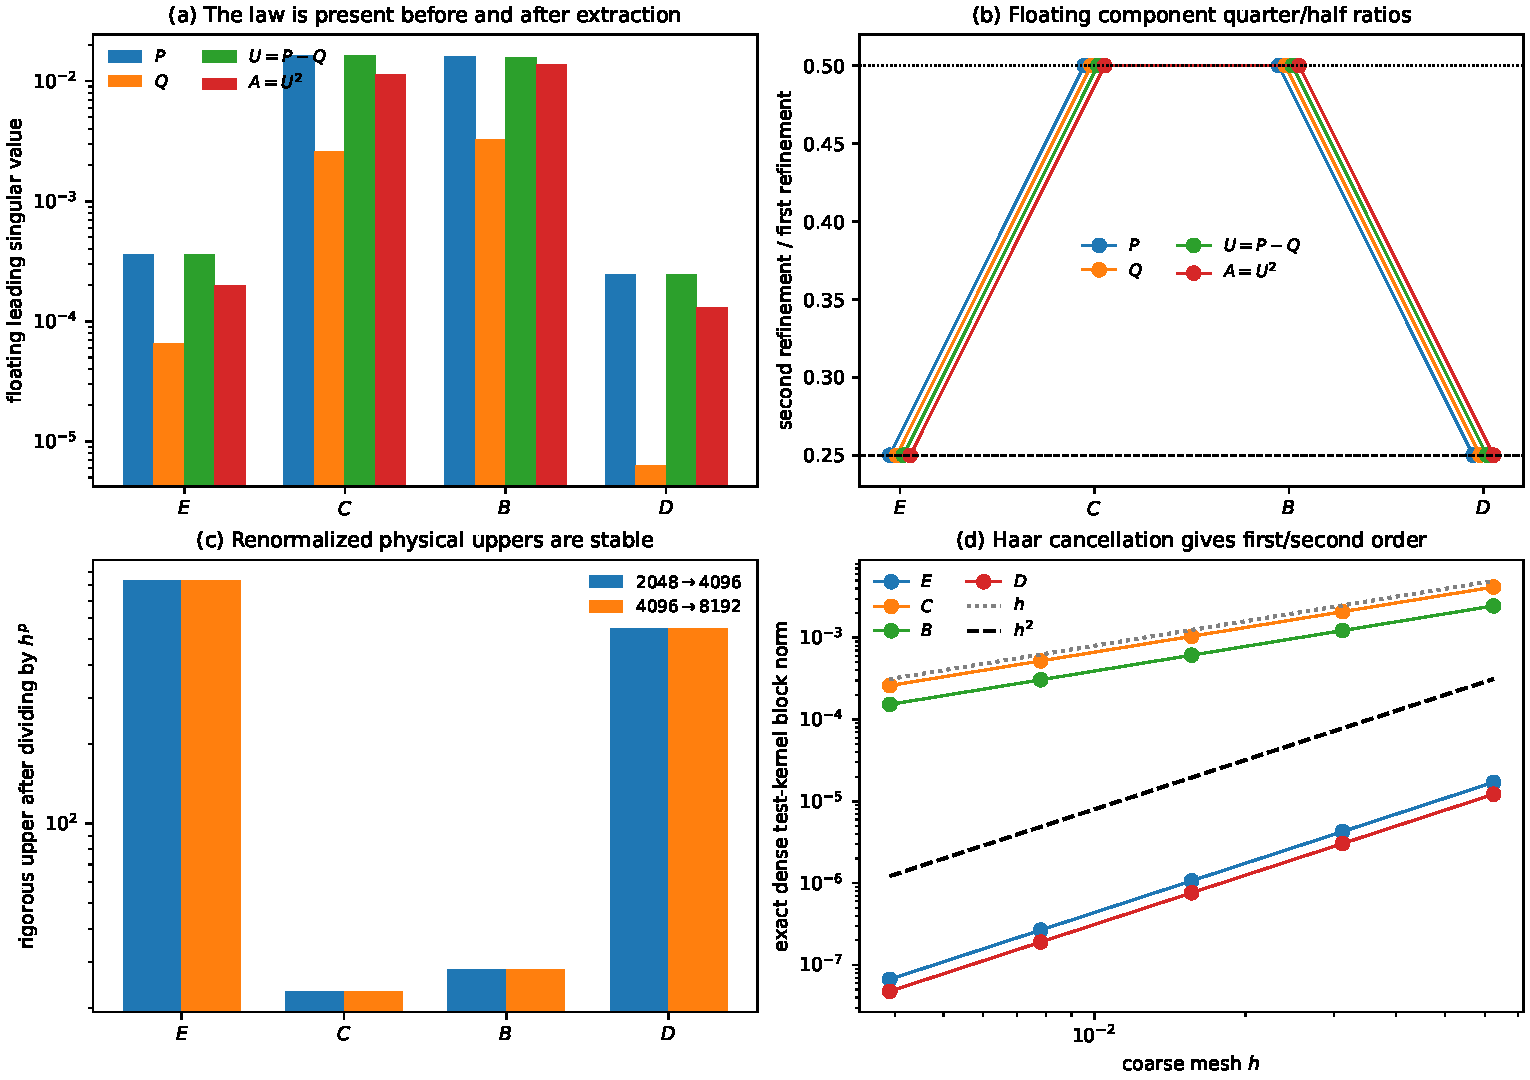
\includegraphics[width=\textwidth]{figures/dyadic_haar_block_decay.pdf}
\caption{Analytic mechanism and finite-scale evidence.  (a) Floating first
refinement block norms for the Markov, peripheral, extracted one-step, and
physical two-step components.  (b) All four component families follow the
quarter--half ratios independently.  (c) The rigorous physical uppers become
nearly level-independent after division by $h^2,h,h,h^2$.  (d) An exact dense
smooth test kernel illustrates the first- and second-order slopes proved in
\cref{thm:haar-decay}.}
\label{fig:summary}
\end{figure}

\section{What is now proved, and what remains}
\label{sec:boundary}

The analytic conclusion is stronger than the original two-point numerical
observation:

\begin{equation}
\boxed{
\text{one Haar difference}=O(h),\qquad
\text{two Haar differences}=O(h^2).
}
\label{eq:boxed-law}
\end{equation}

It survives the three operations that define the intended physical family:
row normalization, smooth finite-rank extraction, and squaring.  Consequently,
if the exact stored sparse/projector family can be placed under the hypotheses
uniformly, its Schur self-energy obeys

\[
\norm{E_h}_2+
\norm{B_h}_2\norm{(z-D_h)^{-1}}_2\norm{C_h}_2=O(h^2)
\]

on any contour whose distance from the vanishing detail spectrum is bounded
below.

This is precisely the perturbative scaling needed by the nested count route.
It is not yet sufficient for an infinite refinement theorem.  Three gates
remain.

\begin{enumerate}[leftmargin=2em]
 \item \textbf{Hard-cutoff defect.}  The eight-sigma sparse support must be
       compared uniformly with the full smooth Gaussian matrix, or the cutoff
       must be allowed to grow with refinement.
 \item \textbf{Peripheral projector enclosure.}  The stored Perron/parity
       projectors must be enclosed relative to a smooth isolated continuum
       spectral projector with an $O(h^2)$ operator bound.
 \item \textbf{Hierarchical resolvent recursion.}  Even when the effective
       perturbation is $O(h^2)$, nonnormal resolvent bounds propagated through
       successive Schur inverses can grow.  Their scalar recursion needs a
       separate summability or bootstrap theorem.
\end{enumerate}

The first two gates connect the exact stored family to the smooth-kernel
theorem.  The third determines whether block decay can be converted into an
all-grid contour-count stabilization result.

\section{Archive and reproducibility}
\label{sec:archive}

The machine-readable certificate records:

\begin{itemize}[leftmargin=2em]
 \item the exact formulas implemented for ideal Haar bounds, discrete
       normalization defects, block squaring, and renormalized constants;
 \item hashes of the inherited RH-36 and RH-37 rigorous block certificates;
 \item the four rigorous physical scaled ledgers and their spreads;
 \item all floating component ratios and effective exponents; and
 \item an explicit list of the theorem's scope limitations.
\end{itemize}

The source tests include exact dense polynomial-kernel checks of all four Haar
inequalities, a quotient-normalization check, and a random dense block-square
check.  The fast replay is

\begin{verbatim}
python -m pytest -q -p no:cacheprovider
python experiments/build_decay_certificate.py
MPLBACKEND=Agg python experiments/make_figures.py
latexmk -pdf -interaction=nonstopmode -halt-on-error main.tex
cp main.pdf dyadic-haar-block-decay.pdf
python experiments/build_archive.py
python experiments/verify_archive.py
\end{verbatim}

The theorem concerns fixed positive noise and smooth full kernels.  It does
not prove the exact sparse all-grid limit, a zero-noise limit, a zeta-zero
identification, a Hilbert--P\'olya construction, or the Riemann hypothesis.

\section{Conclusion}

The quarter--half law seen in two large stored refinements has a simple and
rigorous origin: one Haar difference extracts one derivative, while two Haar
differences extract a mixed second derivative.  Midpoint consistency and the
pure detail block are therefore second order; the cross channels are first
order.  Discrete row normalization, smooth spectral extraction, and operator
squaring preserve those powers.

The physical certificate ledgers agree with the theorem to high precision
after the predicted renormalization, and the component decomposition shows
that the law is already present in both the Gaussian Markov kernel and the
peripheral projector.  The maze is therefore narrower: the next obstruction
is no longer the block scaling itself, but a uniform cutoff/projector bridge
and control of the resulting multilevel resolvent recursion.

\bibliographystyle{plainnat}
\bibliography{references}

\end{document}
